\documentclass[UTF8]{ctexart}
\usepackage{CJKutf8}
\usepackage{listings}
\usepackage{geometry}
\usepackage{xcolor}
\usepackage{graphics}
\usepackage{graphicx}
\lstset{
	backgroundcolor=\color{white},
	basicstyle=\footnotesize\ttfamily,
	breakatwhitespace=false,
	breaklines=true,
	captionpos=b,
	commentstyle=\color{mygreen},
	deletekeywords={...},
	escapeinside={\%*}{*)},
	extendedchars=true,
	frame=single,
	keepspaces=true,
	keywordstyle=\color{blue},
	morekeywords={*,...},
	numbers=left,
	numbersep=5pt,
	numberstyle=\tiny\color{gray},
	rulecolor=\color{black},
	showspaces=false,
	showstringspaces=false,
	showtabs=false,
	stepnumber=4,
	stringstyle=\color{purple},
	tabsize=4,
	title=\lstname
}
\geometry{a4paper, left=1cm, right=1cm}
\title{操作系统实验报告}
\author{顾芃骐20079100001}
\begin{document}
	\maketitle
	\newpage
	\section{进程的建立}
	\begin{itemize}
		\item 实验目的:学会通过基本的Windows或者Linux进程控制函数,由父进程创建子进程,并实现父子进程协同工作。
		\item 实验软件环境:Ubuntu22.04 \& GNU-C++17
		\item 实验内容:创建两个进程,让子进程读取一个文件,父进程等待子进程读取完文件后继续执行,实现进程协同工作。进程协同工作就是协调好两个进程,使之安排好先后次序并以此执行,可以用等待 函数来实现这一点。当需要等待子进程运行结束时,可在父进程中调用等待函数。
	\end{itemize}
	\subsection{代码实现}
    在“\textbf{\textit{os1.cpp}}”中写如下代码,并创建名为“\textbf{\textit{os1.in}}”的文件,在后者中写入且仅写入“TextMessage”作为测试输出内容。
\begin{lstlisting}[language=c++]
#include<fstream>
#include<unistd.h>
#include<stdio.h>
#include<iostream>
using namespace std;
int main(){
	int flag = 0;
	string answer = "";
	auto x = vfork();
	if (!x) {
		ifstream in("os1.in");
		in >> answer;
		in.close();
		flag = 1;
		cout << "End of Child Process" << endl;
	} else {
		while (!flag);
		cout << "Start of Main Process" << endl;
		cout << answer << endl;
		cout << "End of Main Process" << endl;
	}
	return EXIT_SUCCESS;
}
\end{lstlisting}
\subsection{实验结果}
运行上述代码,可得到如下左图所示的实验结果。片刻之后,终端显示如右所示的结果。
\begin{center}
        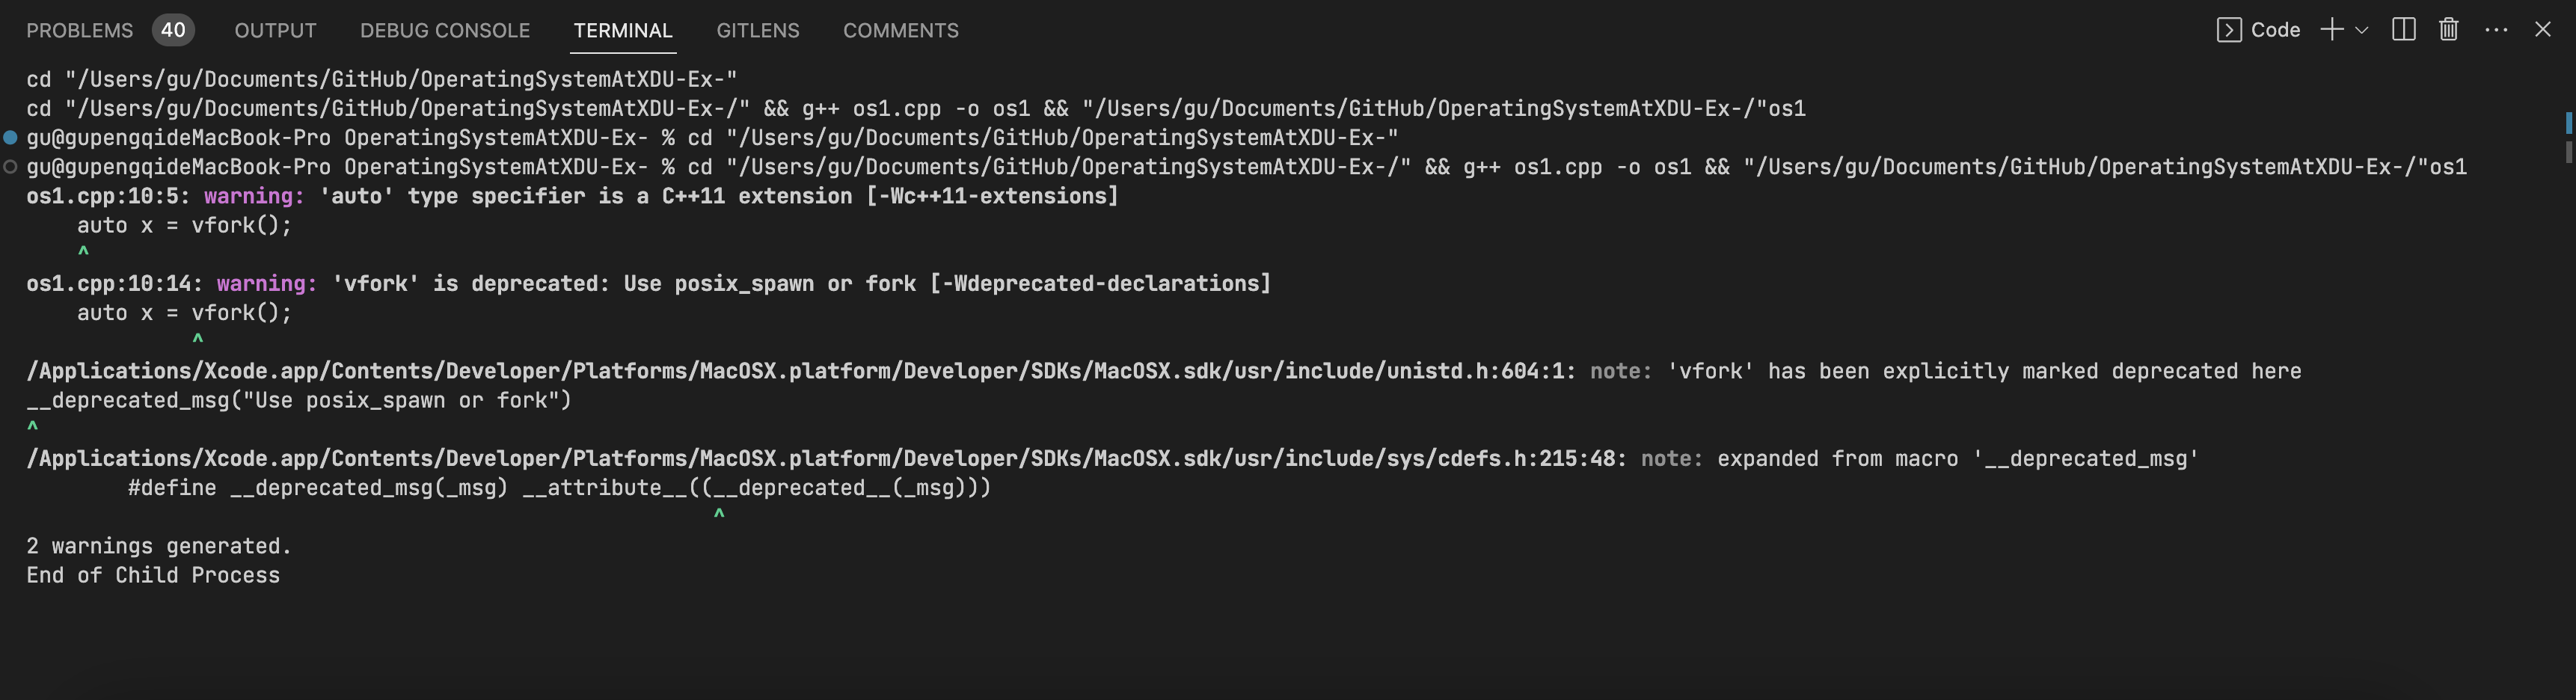
\includegraphics[width=0.3\pdfpagewidth]{os1-1.png}
        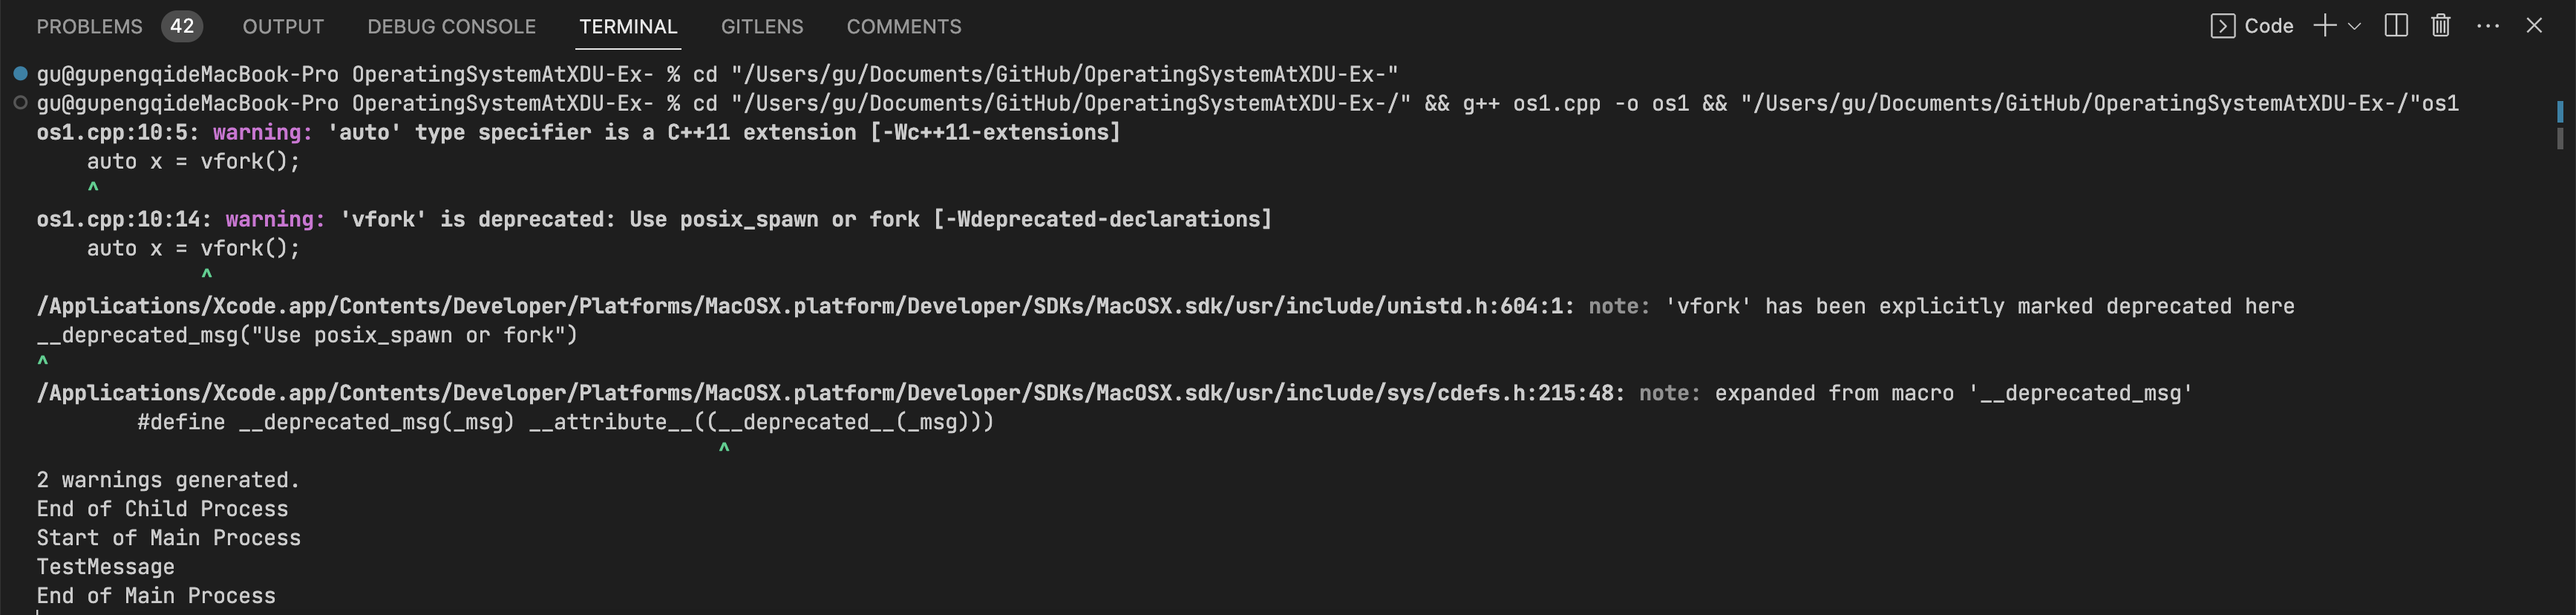
\includegraphics[width=0.3\pdfpagewidth]{os1-2.png}
\end{center}
\subsection{实验结果分析}
在1.1所示代码中,子进程读取了文件“\textit{os1.in}”;读取完成后,父进程继续执行,并显示了开始、结束和子进程所读取的文件内容。需要注意的是,使用\texttt{vfork}时修改静态区变量是未定义行为,会引发“栈溢出(stack smashing)”。
\end{document}